\section{Execution}
\label{sec:Durchführung}

The apparate is constructed as seen in \autoref{fig:apparate}.

\begin{figure}[H]
    \centering
    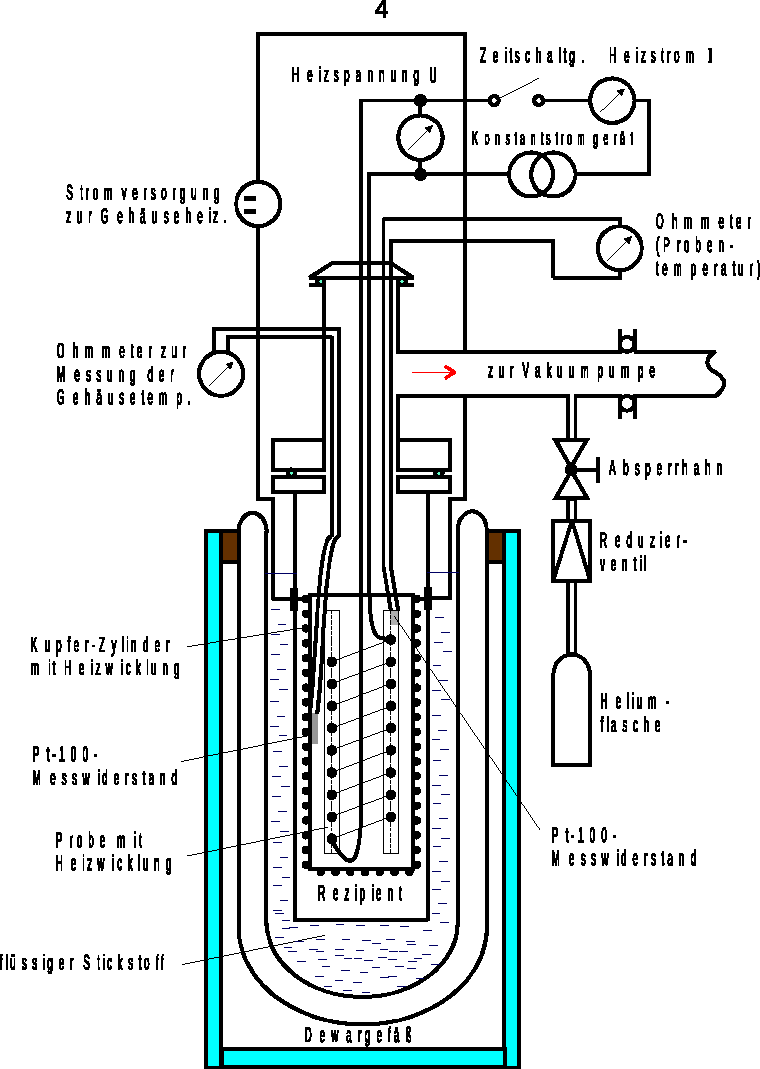
\includegraphics[]{figures/apparature.pdf}
    \caption{Schematic representation of the used apparate \cite{v47}.}
    \label{fig:apparate}
\end{figure}

It consists of a cryogenic storage dewar that isolates the apparate from its surroundings. Inside the dewar, there is a copper cylinder encased inside a recipient.
The recipient is hooked up to a vacuum pump, so that any air may be pumped out in order to prevent heat transfer through convection and a bottle of helium that is used to aid the cooling process.
The copper cylinder itself is outfitted with a heat spiral.
Both the copper cylinder's and the recipient's temperatures can be monitored via Pt-100-Resistances. \\

Firstly, all air inside the recipient is pumped out so that any potential moisture is removed. That is to prevent the build up of frost on the copper cylinder which might negatively impact the heating process. \\
Then, the vacuum pump is turned off, helium is let inside the recipient and nitrogen is added to the dewar.
The nitrogen then cools down the recipient which in turn cools the copper via the helium.
During the cooling process, the temperature of both shell and sample is monitored via the Pt-100s until a resistance of around $22 \,\si{\ohm}$ is reach, equating to a temperature of around $-190 \,\si{\celsius}$. \\

Next, the copper is heated again. For that, the helium is pumped out via the vacuum pump and a heating current of $160 \si{\milli\ampere}$ is applied to the copper.
Then, the time intervals for a change in temperature of $\Delta T = 10 \,\si{\celsius}$ are measured until the sample reaches a temperature of around $10 \,\si{\celsius}$.
During that time, an additional heating current is applied to the recipient, keeping it close to the sample's temperature to make sure that radiative heat transfer between the two remains as small as possible.